\section{The Emotiv\textsuperscript{®} EPOC+}
\begin{figure}[htbp]
	\centering
		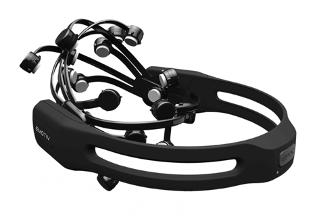
\includegraphics[width=0.5\columnwidth]{epoc.png}
	\caption{Emotiv EPOC+ Headset}
	\label{fig:epoc}
\end{figure}

Although easily modifiable, the MusEEG package is designed to work with the Emotiv\textsuperscript{®} EPOC+. The EPOC+ is an affordable commercial-grade EEG headset that records 14 EEG channels and samples at a rate of 256Hz with 14-bit resolution, with a least significant bit value of approximately 0.51 $\mu$V. The EPOC+ headset proves to be an economically feasible alternative to a medical-grade headset as various studies confirm its viability for noncritical applications \cite{10, 11, 12, 13}.  

\section{Data Acquisition}
To maximize classification accuracy, the MusEEG package is designed with a train-it-yourself structure, meaning that the end-user will have to train their own ANN model to work with their preferred set of facial or body expressions. Because of the train-it-yourself nature of the package, data was recorded for a single subject only. Six facial expressions were recorded using the Emotiv\textsuperscript{®} PRO application. 80 samples were recorded of the following facial expressions: 
\begin{itemize}
\item smile
\item raise eyebrows
\item look left
\item look right
\item neutral
\item scrunch
\end{itemize}

To expedite recording times, the MusEEG package was designed to allow the user to record all samples of a single facial expression to a single .csv file. The MusEEG package then aids the user through curating and cutting the samples into individual chunks for feature extraction and classification. 

\begin{figure}[htbp]
	\centering
		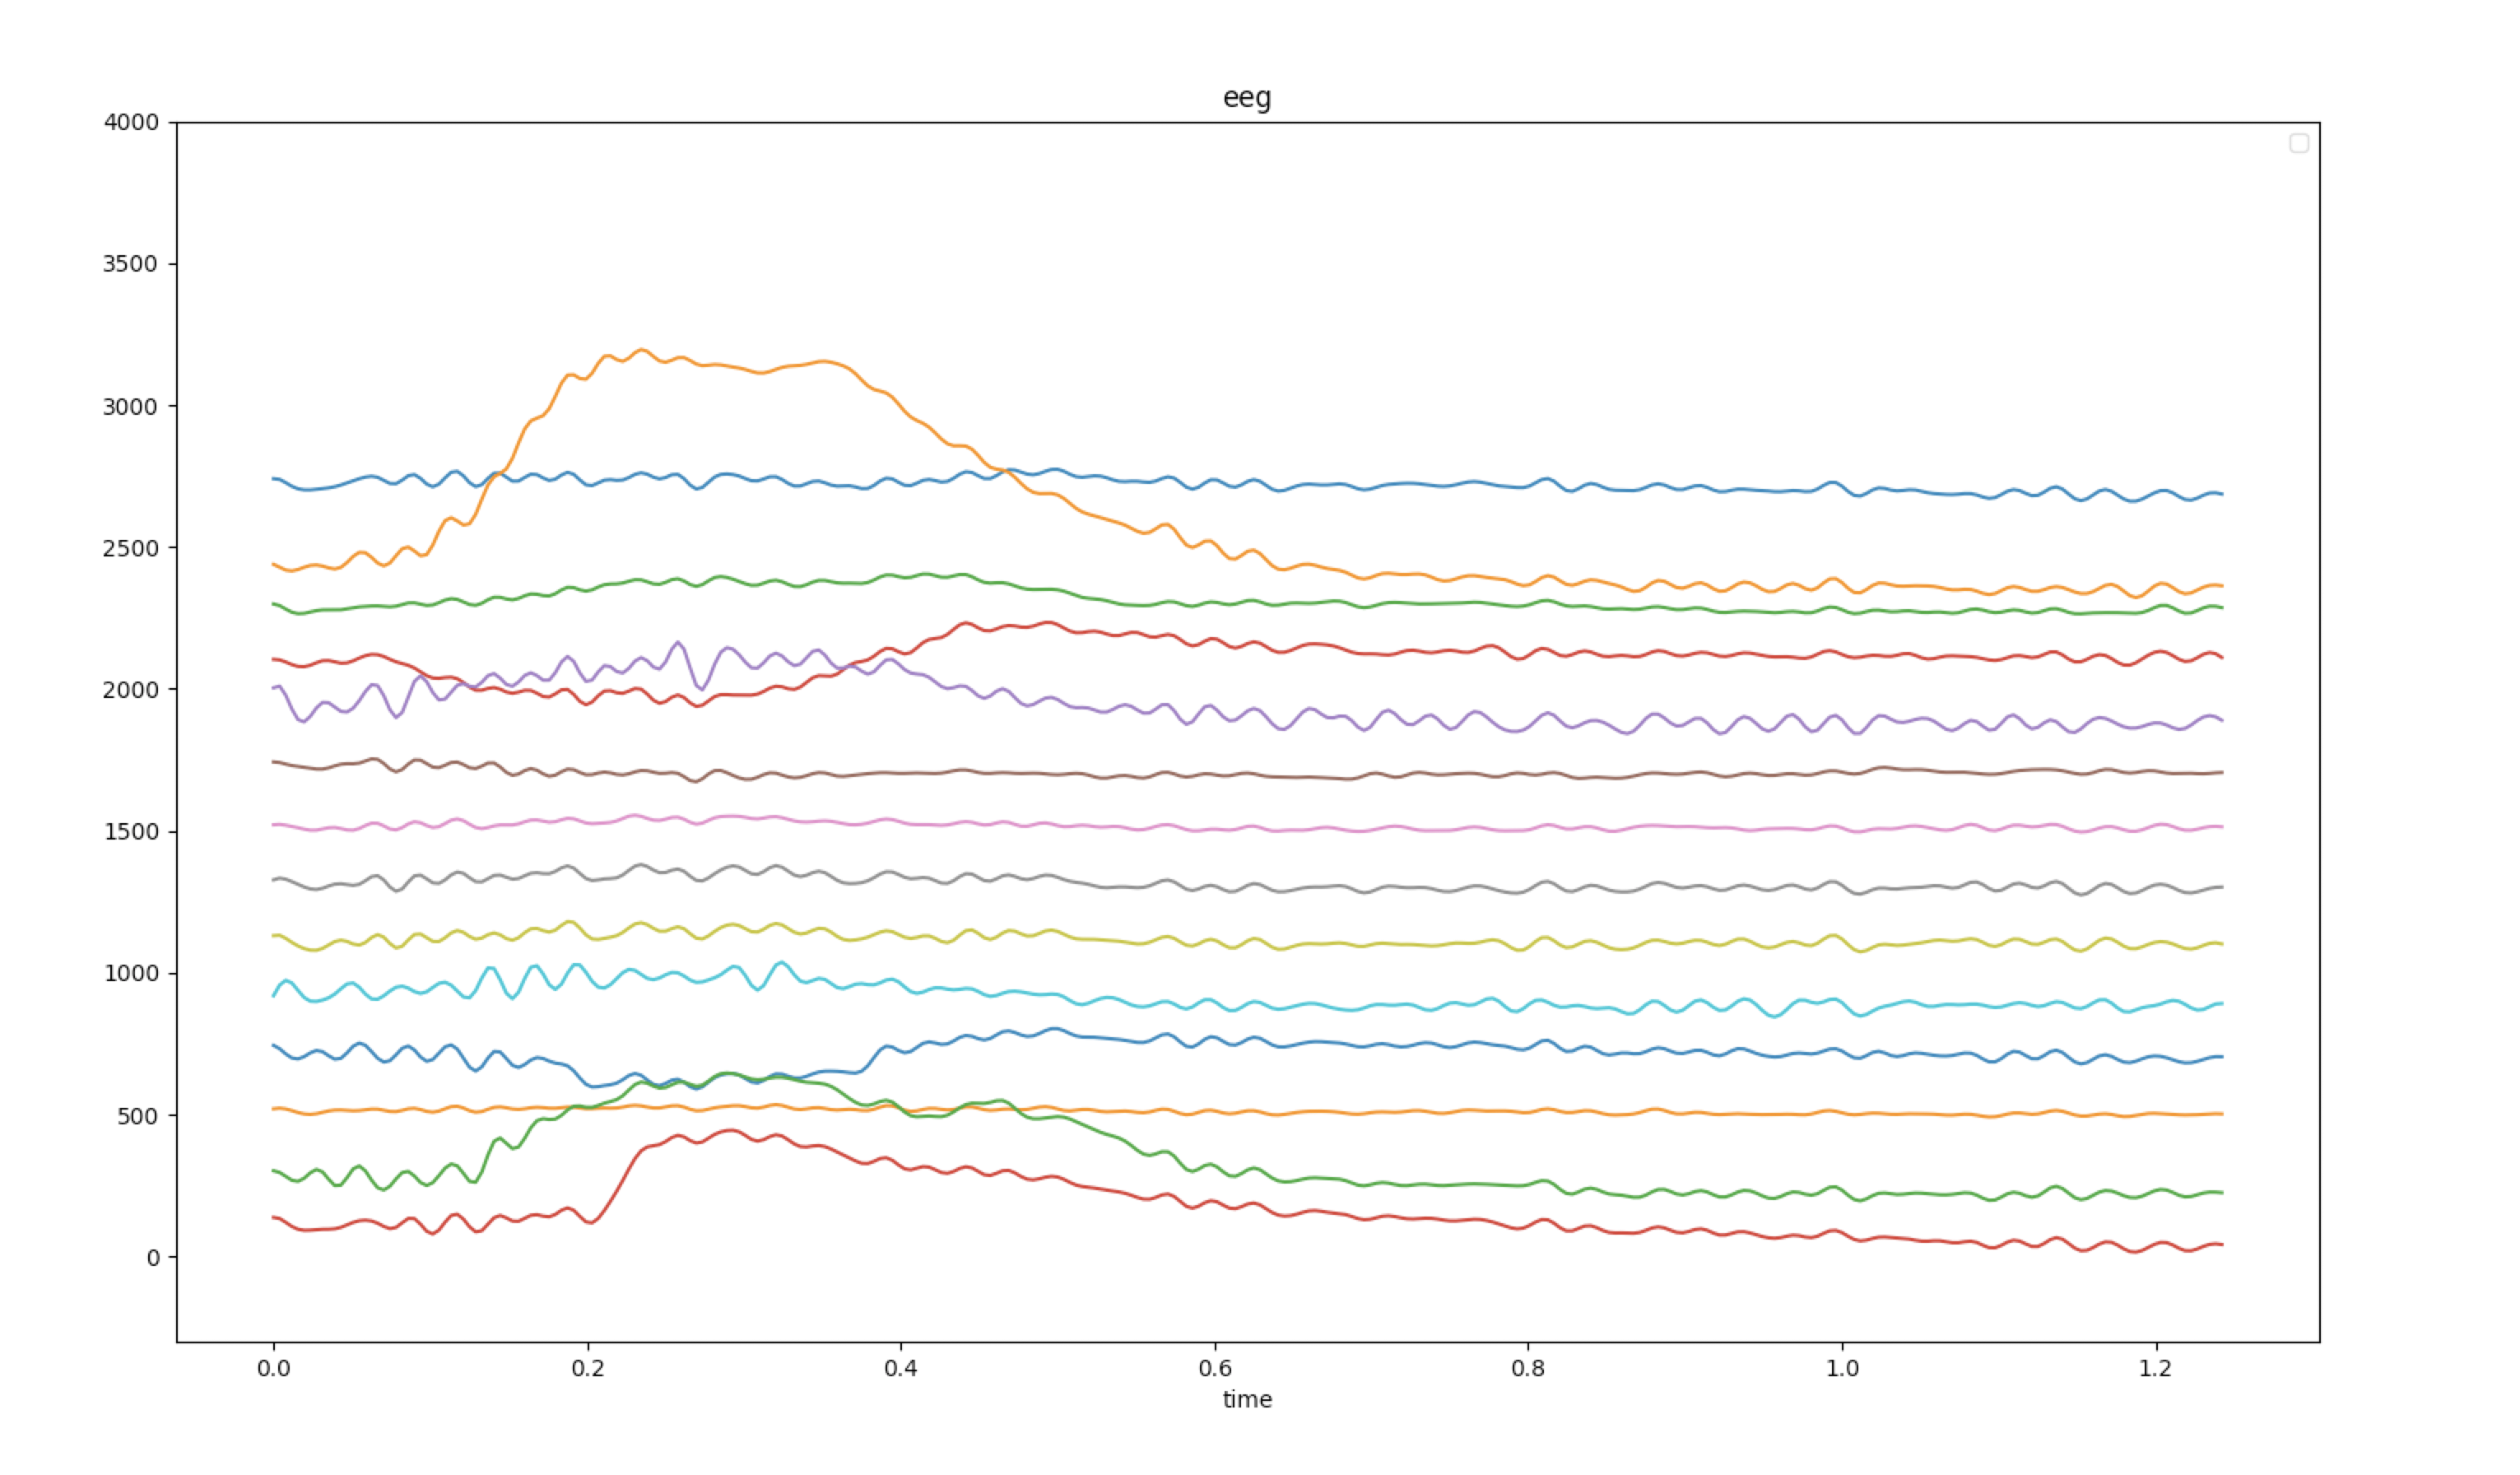
\includegraphics[width=1\columnwidth]{smileBigChunk_320.png}
	\caption{EEG plot of a smile sample (\textit{bigChunk})}
	\label{fig:smileBigChunk}
\end{figure}

During the curation process, the samples were examined for any discontinuities in contact quality, noise, and other artifacts. Samples that appeared to be corrupted with electrode contact discontinuities were discarded, while samples that were clean were stored in the project’s saved chunks directory. From each sample, two different sample chunks were created: a \textit{bigChunk} (1250ms, 320 samples) for facial expression recognition, and a \textit{smallChunk} (250ms, 64 samples) for facial expression/no facial expression classification. Examples of a \textit{bigChunk} and \textit{smallChunk} can be observed in (Figures~\ref{fig:smileBigChunk} and \ref{fig:smileSmallChunk}), respectively.

\begin{figure}[htbp]
	\centering
		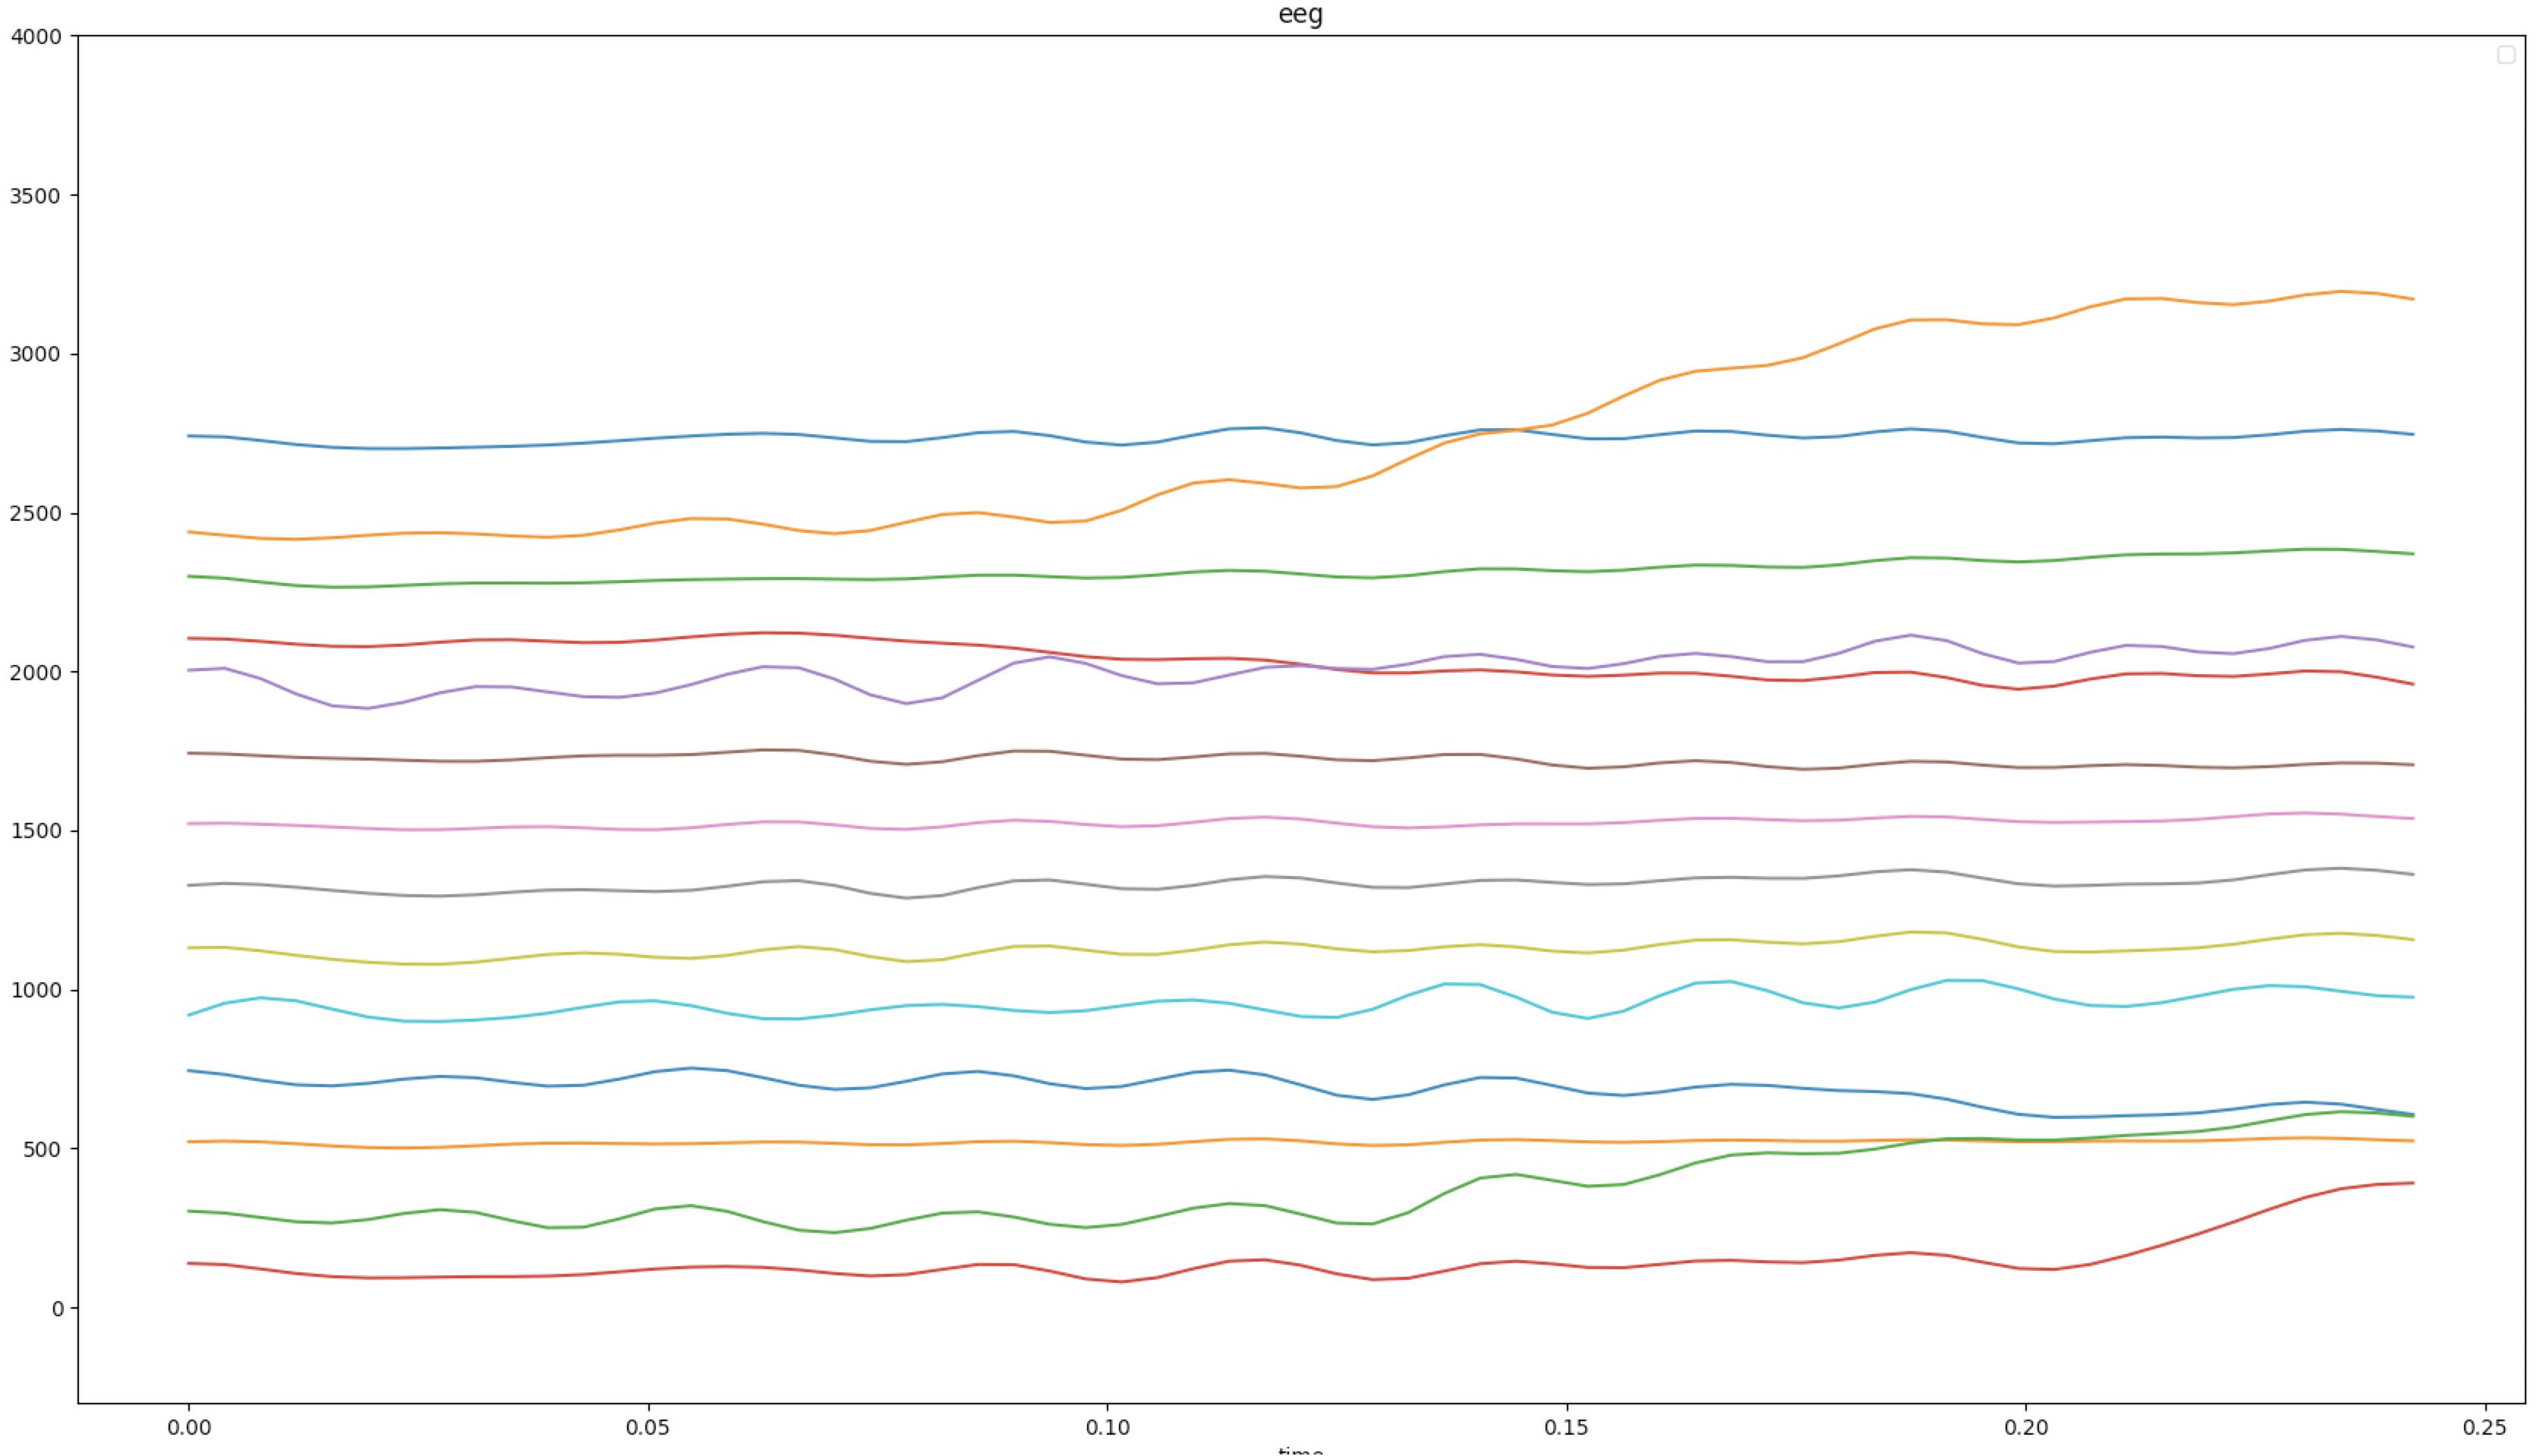
\includegraphics[width=1\columnwidth]{smileSmallChunk_64.png}
	\caption{EEG plot of a smile sample (\textit{smallChunk})}
	\label{fig:smileSmallChunk}
\end{figure}

\section{Feature Extraction}
\subsection{Facial Expression Feature Extraction}
A feature extraction method similar to the one in \cite{14} was used. A 4-level wavelet decomposition using Daubechies order-2 (db2) mother wavelet is performed on all 14 channels of the chunk of EEG data.

One advantage of wavelet analysis over other time-frequency distribution methods (e.g. STFT) is that wavelet analysis varies the time-frequency aspect ratio, producing good frequency localization at low frequencies (long time windows) and good time localization at high frequencies (short time windows). This results in a segmentation of the time-frequency plane that will reveal transient features of the signal, which are typically not obvious during Fourier analysis \cite{14}. 

Following the wavelet decomposition, the first four statistical moments (mean, variance, skewness, kurtosis) are calculated for each wavelet vector. Since four moments are calculated for each of the 5 wavelet decomposition vectors per EEG channel, a total of 14 x 4 x 5 (280) features are calculated. The data is then normalized using \textit{sklearn}'s MinMaxScaler. These features are used as an input for the classification models.
 
\begin{figure}[htbp]
	\centering
		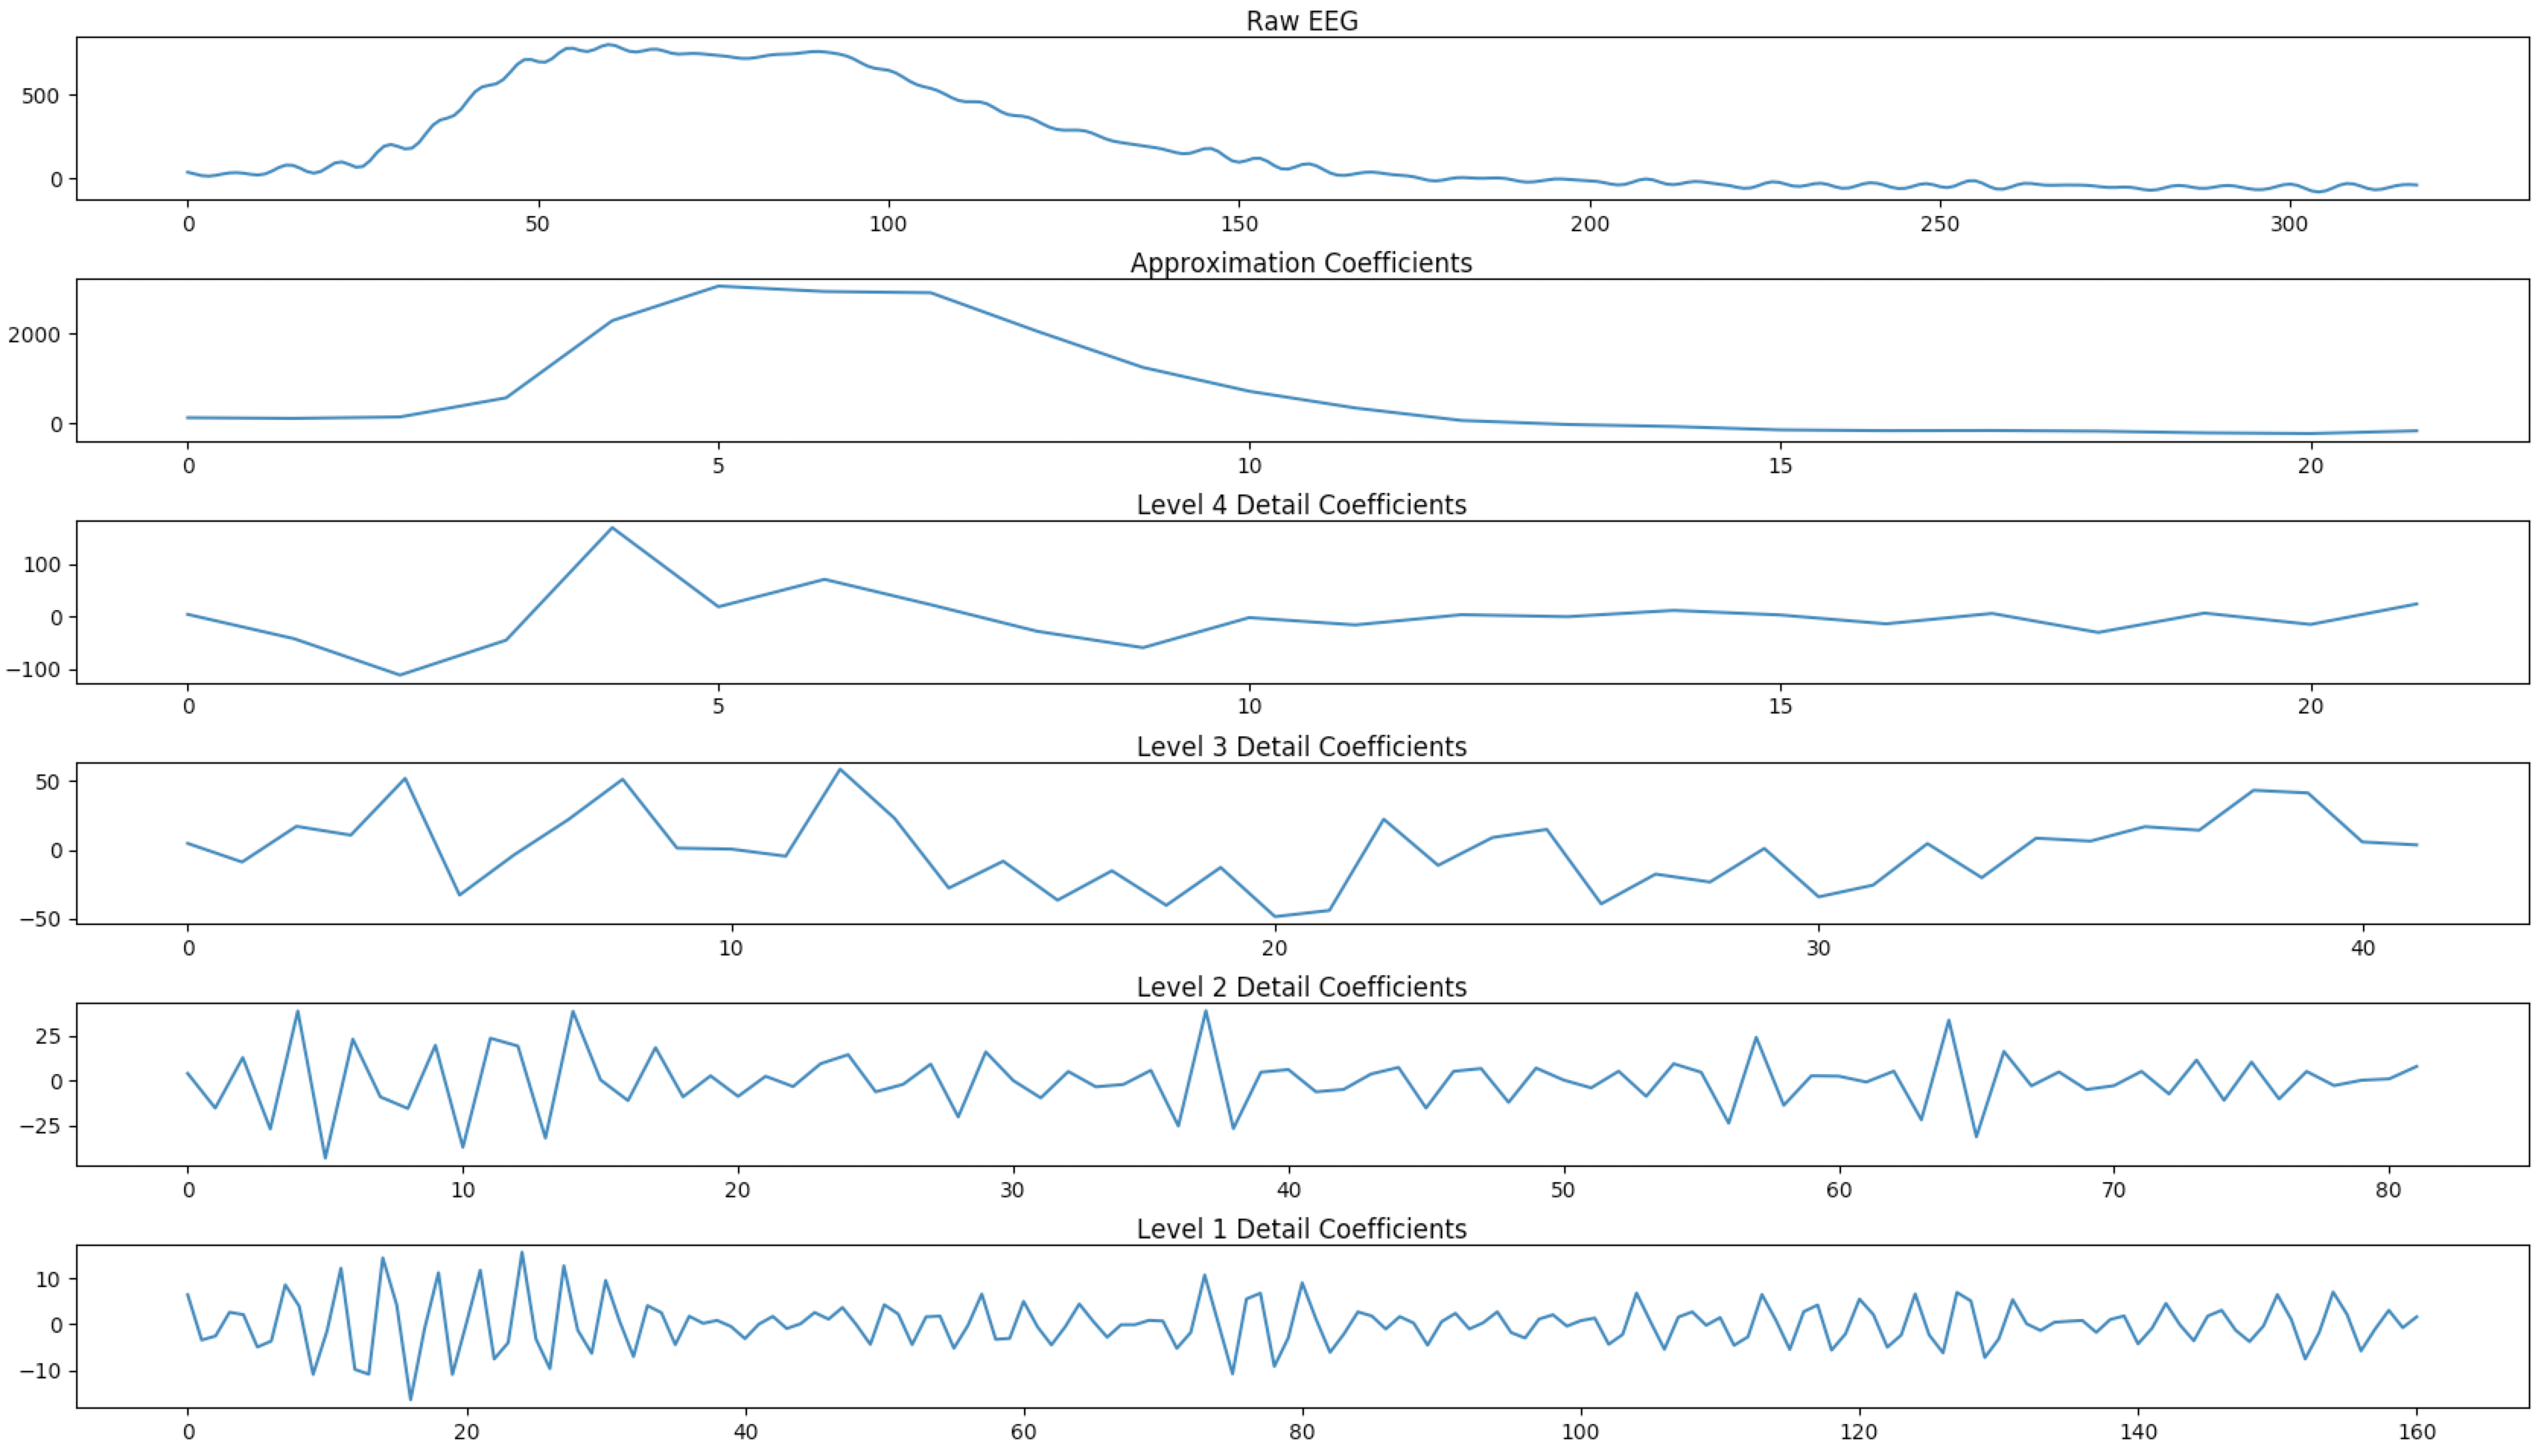
\includegraphics[width=1\columnwidth]{smileWavelets.png}
	\caption{Wavelet coefficients plot for smile}
	\label{fig:smileWavelets}
\end{figure}

\subsection{Band Power Feature Extraction}
The MusEEG system is capable of sending continuous theta (4 - 8 Hz),  alpha (8 - 12 Hz), beta (12 - 30 Hz), and gamma (30  - 60 Hz) band power information at a rate of 2Hz. 

\begin{figure}[htbp]
	\centering
		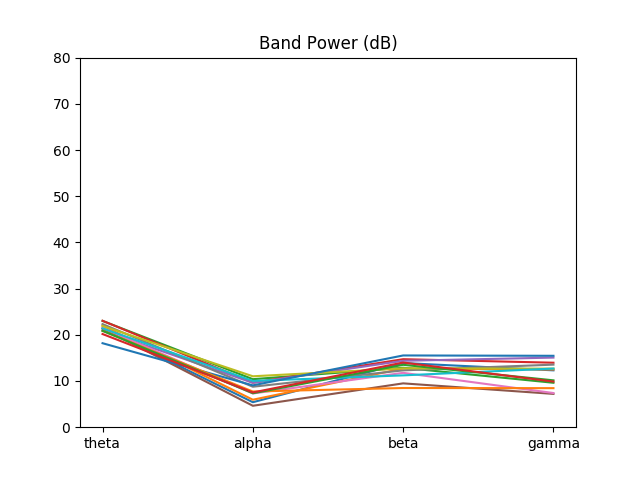
\includegraphics[width=0.8\columnwidth]{bandPower.png}
	\caption{EEG band power during neutral state}
	\label{fig:bandpower}
\end{figure}

Before the average band power is calculated, the power spectral density of all of the 14-channel data is calculated using Welch's periodogram, with a window duration of 0.5s. Once the power spectral density is calculated, the average band power over a certain range of frequencies is found by integrating the power spectral density over the frequency ranges. 

\section{Classification}
A three-layer Artificial Neural Network (ANN) architecture was used for the classification of the EEG signals. Two models were created: a small model designed to analyze 64-sample chunks and determine whether the chunk contains a facial expression or not (\textit{smallBrain}), and a large model designed to analyze 320-sample chunks to determine what facial expression is present in the chunk (\textit{bigBrain}).

The \textit{smallBrain} model is meant to perform a quick classification of whether a facial expression is present in a 64-sample chunk. The \textit{smallBrain} model was designed with the intent of having an always-on processor for real-time implementation. By analyzing a chunk with a duration of 250ms, the \textit{smallBrain} model returns a result fairly quickly, allowing for continuous real-time classification with little latency.

\begin{figure}[htbp]
	\centering
		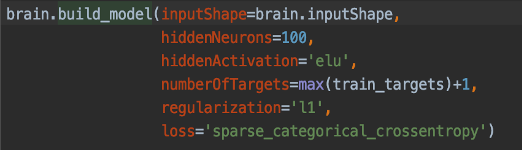
\includegraphics[width=1\columnwidth]{smallBrain.png}
	\caption{ANN architecture for \textit{smallBrain} model.}
	\label{fig:smallBrain}
\end{figure} 

\begin{figure}[htbp]
	\centering
		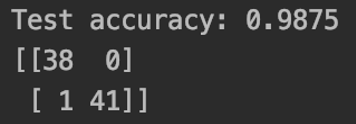
\includegraphics[width=0.5\columnwidth]{smallBrainConfusion.png}
	\caption{Confusion Matrix for \textit{smallBrain} model.}
	\label{fig:smallBrainConfusion}
\end{figure} 


The \textit{smallBrain} model consists of a three-layer ANN with L1 regularization methods and a sparse categorical cross entropy loss function. During testing, the model exhibited 98.75\% accuracy. Its test confusion matrix can be observed in (Figure~\ref{fig:smallBrainConfusion}) .


The \textit{bigBrain} model consists of a three-layer ANN with L1\_L2 regularization methods and a sparse categorical cross entropy loss function.  During testing, the model exhibited 87.04\% accuracy. Its test confusion matrix can be observed in (Figure~\ref{fig:bigBrainConfusion}).

\begin{figure}[htbp]
	\centering
		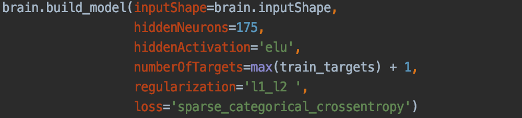
\includegraphics[width=1\columnwidth]{bigBrain.png}
	\caption{ANN Architecture for \textit{bigBrain} model.}
	\label{fig:bigBrain}
\end{figure} 

 \begin{figure}[htbp]
	\centering
		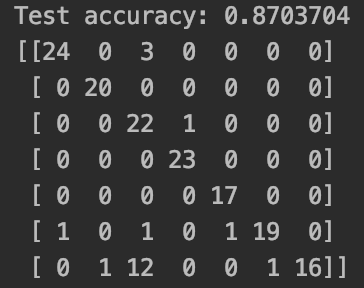
\includegraphics[width=0.75\columnwidth]{bigBrainConfusion.png}
	\caption{Confusion Matrix for \textit{bigBrain} model.}
	\label{fig:bigBrainConfusion}
\end{figure} 